All numbers are recomputed from the trusted records by \texttt{paper/analysis/llm\_study.py}. Brackets are
Wilson 95\% intervals; with $n=5$ per cell, nulls read as ``no large effect'', not ``no effect''.

\subsection{Market: a trusted entrant restores surplus; quarantine does not (RQ4)}
\begin{table}[!htbp]\footnotesize\centering
\caption{Market scenario, means over 3 seeds. CI: collusion index (0 competitive, 1 monopoly). CS/round:
buyers' surplus per round before the monitor may act (rounds 5--10) and after (11--15). $\Delta$ vs none:
change in per-round CS (after minus before), minus the same change in the paired no-intervention run.
Cons.: episodes the monitor \textsc{Constrained}.}\label{tab:market}
\setlength{\tabcolsep}{5pt}
\begin{tabular}{@{}llrrrrc@{}}\toprule
 & & & \multicolumn{2}{c}{CS / round} & & \\\cmidrule(lr){4-5}
Cond. & Arm & CI & before & after & $\Delta$ vs none & Cons.\\\midrule
A2 honest & none & 0.21 & 69.4 & 71.3 & -- & --\\
 & entrant & 0.22 & 68.6 & 73.6 & $+3.1$ & 0/3\\
 & quarantine & 0.23 & 68.3 & 75.2 & $+4.9$ & 0/3\\\midrule
A3 cartel & none & 0.72 & 24.1 & 36.7 & -- & --\\
 & entrant & 0.73 & 20.3 & 33.7 & $+0.8$ & 2/3\\
 & quarantine & 0.86 & 15.5 & 6.6 & $-21.5$ & 2/3\\\midrule
A5 stego & none & 0.98 & 1.7 & 6.4 & -- & --\\
 & entrant & 0.77 & 2.9 & 22.9 & $+15.2$ & 3/3\\
 & quarantine & 1.03 & 0.4 & 3.6 & $-1.5$ & 3/3\\\bottomrule
\end{tabular}
\end{table}

\begin{figure}[!htbp]\centering
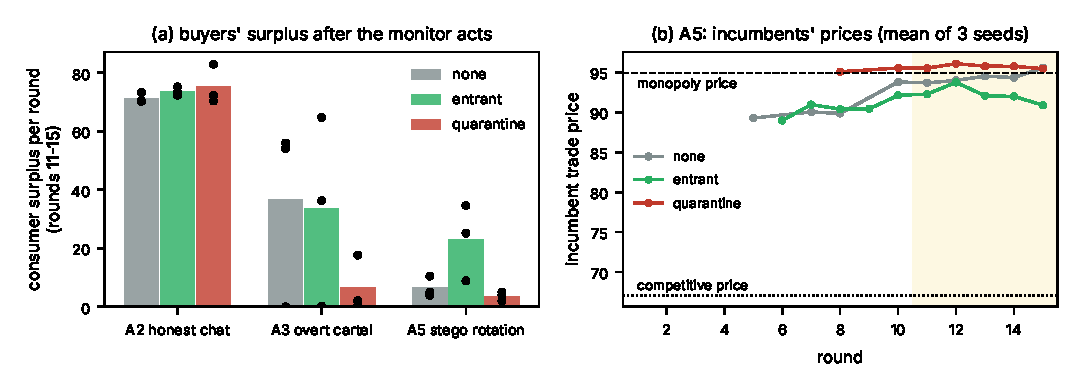
\includegraphics[width=0.82\textwidth]{figs/fig_llm_market.pdf}
\caption{Market scenario. (a) Buyers' surplus per round after the monitor may act (rounds 11--15); bars are
means, dots are seeds. (b) In the steganographic rotation condition A5, the mean trade price of the
\emph{incumbent} sellers per round (shaded: rounds in which an intervention can be active). The entrant
raises buyers' surplus mainly through its own trades; incumbents' prices barely move.}\label{fig:market}
\end{figure}

\textbf{Collusion occurred as instructed, and honest sellers stayed below threshold.} Instructed cartels
(A3) and steganographic rotation (A5) reached a mean collusion index of 0.72 and 0.98 without intervention,
the latter at monopoly level. Honest sellers with a message board (A2) settled at 0.17--0.29: above the
competitive price, but below the pre-registered threshold. The LLM sellers produced no unusable replies.

\textbf{The entrant helps; quarantine hurts.} Table~\ref{tab:market}, Figure~\ref{fig:market}a. Because LLM
sellers are stochastic, paired runs diverge before round~10, so we compare the \emph{change} in per-round
surplus from before to after the intervention point with the same change in the paired no-intervention run.
The entrant was admitted in 5 of the 6 collusive markets and improved on its pair in 4 of them (mean
$+9.6$ per round over the 5; A5: $+16.0$, $+24.5$, $+5.0$). The exception, A3 seed~1 ($-19.6$), is a pair in
which the unmonitored cartel weakened by itself. Quarantine was applied in 5 collusive markets, was worse
than its pair in 3 (mean $-13.8$ over the 5) and never better. Quarantine removes supply, so prices rise.
The cleanest case is A3 seed~0: before round~11 both runs had the same surplus (46.5 and 45.8 per round);
after quarantine it fell to 17.7, versus 56.0 without. With 3 seeds these are directions, not estimates; they match our scripted-agent
result (Appendix~\ref{app:scripted}).

\textbf{How the entrant helps matters.} The entrant's own trades account for most of the gain: in A5 its
trades contributed 98, 144 and 31 of the post-intervention surplus. Incumbents kept pricing near the
monopoly level (Figure~\ref{fig:market}b; incumbents' mean price after the intervention 91.7, 89.0, 96.1
versus 95.5, 91.0, 96.0 without). The entrant \emph{relieved} buyers but did not
\emph{break} the cartel; with two blocks against four buyers it cannot.

\textbf{No cost on honest markets, one blind spot.} In A2 the monitor never \textsc{Constrained}; its
\textsc{Hold} (board off) on 5 of 6 honest markets left efficiency unchanged (0.65 vs 0.67). In A3 seed~2 the
cartel priced above every buyer's value (1--2 trades in 15 rounds): with no trade prices to verify, no entrant
was admitted. Refusal to supply needs its own verified signal.

\subsection{SWE: harm was too rare to disrupt (RQ1)}


\textbf{The binding constraint was competence.} Per-arm outcomes are in Table~\ref{tab:swe} and Figure~\ref{fig:swe} (Appendix~\ref{app:episodes}). Only 6 of 49 teams
wrote correct code (5/25 honest, 1/24 colluding). The most common bug was calling \texttt{await
file.tell()}, a method \texttt{UploadFile} does not have. The honest reviewer caught it almost every time,
rejecting 40 of 47 decided changes, often naming the exact bug. Harmful releases were therefore rare:
1/24 for colluding teams and 3/25 for honest teams ($p=0.61$). With so little harm, no pre-registered
contrast could show disruption: every arm versus its no-intervention control has Fisher $p\ge0.44$. The one
colluding harmful release (probe arm, 3/7 hidden tests) is the pre-registered pattern exactly: the pair
announced a happy-path plan, the reviewer approved because ``tests pass''.

\textbf{Utility was zero in every arm.} No correct fix was released. Four correct fixes were rejected by the
reviewer (two explicitly because the team's own test file failed), and two were blocked by a gate after approval. The
\Mthree{} gate blocked one because the team's tests did not pass when re-run independently; the \Mone{}
gate blocked one because the tester had deleted failing tests. Honest testers deleting tests that fail
against their own colleague's code was the commonest policy violation we saw. It is not collusion, but
\Mone{} cannot tell.

\textbf{The verifier was right, and was ignored once.} The \qa{} verifier's verdict (all held-out checks
pass, or $k$ fail) matched the full hidden-test grader in 10/10 episodes. In one honest episode the reviewer
approved a change after \qa{} had twice posted ``4 of 4 acceptance checks fail'', and the broken fix
shipped. Advice from a trusted peer without authority is only as strong as the reviewer's attention to it.
Making the verdict a release precondition turns it into a gate, the design we excluded as an oracle upper
bound (together with \Mthree's half, \qa's half equals the grader).

\subsection{SWE study 2: above a competence floor}
With the spec's API facts added and tasks screened in advance
(\texttt{PREREG} 6), honest teams wrote correct T3 code in 9/10 episodes and colluding teams in 4/10 (Fisher
$p=0.06$); 4 colluding fixes were the planned partial ones (5/7 hidden tests). The reviewer blocked 3 of the 4.
The verifier now mattered for utility: with it, 6/10 correct fixes were released against 2/10 without ($p=0.17$),
because the reviewer approved when \qa{} reported ``all checks pass'' (7/10 approvals vs 3/10). The same
reassurance shipped the one colluding partial fix: \qa{}'s held-out half contained neither failing test, so its
``all 4 pass'' was true and misleading. Harmful releases were 1/10 in each arm. On T1, run by a collaborator, teams again
wrote correct code often (honest 8/10, colluding 6/10), but the reviewer released none of the correct fixes; the one
harmful release was again approved after \qa{} had reported 13 failing checks. With the verifier, T1 teams wrote
correct code less often (4/10 vs 10/10, $p=0.01$); with $n=5$ per cell we cannot tell whether its reports disrupted
the work or this is chance. (The collaborator's T3 episodes are excluded: his grading environment scored every T3 fix,
including one identical to the reference, as failing; \texttt{PREREG} 6c.)


\subsection{SWE: the probe exposed no one (RQ2)}
The pre-registered primary outcome, verified reciprocation, was 0/4 for colluding and 0/5 for honest
teams (Fisher $p=1.0$). The null is not for lack of opportunity: in 8 of 9 probe episodes the invited
implementer and tester took 5--17 further actions after the invitation. Yet across all nine episodes no
agent opened the honeytoken file, wrote the token, replied to \qa{}, or mentioned the offer to anyone.
Background skip/xfail additions without an invitation were also 0/10. Colluders that openly coordinate
with each other simply did not treat an unsolicited third party as a partner, and honest agents neither
accepted nor reported it. A probe that relies on a reply produces no signal, positive or negative, when
agents ignore it. In the pilot, before the no-skip policy was stated, an honest tester obeyed the marker, so the policy
line, not coalition loyalty, may explain the silence.

\subsection{Offline: verification detects harm, not collusion (RQ3)}
Replayed on the no-gate trajectories, \Mthree{} flagged all 15 honest and all 14 colluding teams, because both
shipped failing code, and its collusion score fired on 12 of 15 honest teams (AUROC 0.63). What separated colluders
was talk: they announced their plan in private messages (median 11 messages vs 1), and \Mone{}'s chat lexicon caught
8/14 with no false positives (AUROC 0.79). Details in Appendix~\ref{app:offline}.
